\section{The Motion of Charged Particles in Magnetic Fields}
When a charged particle passes through a magnetic field, we can separate the motion into two components. 
\begin{center}
    \tikzset{every picture/.style={line width=0.75pt}} %set default line width to 0.75pt        

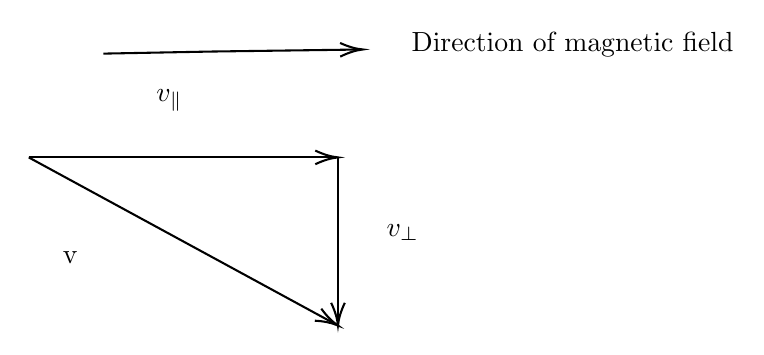
\begin{tikzpicture}[x=0.75pt,y=0.75pt,yscale=-1,xscale=1]
%uncomment if require: \path (0,300); %set diagram left start at 0, and has height of 300

%Straight Lines [id:da42319733275995863] 
\draw    (252,126) -- (399,126) ;
\draw [shift={(401,126)}, rotate = 180] [color={rgb, 255:red, 0; green, 0; blue, 0 }  ][line width=0.75]    (10.93,-3.29) .. controls (6.95,-1.4) and (3.31,-0.3) .. (0,0) .. controls (3.31,0.3) and (6.95,1.4) .. (10.93,3.29)   ;
%Straight Lines [id:da8555331334957245] 
\draw    (401,126) -- (401,205) ;
\draw [shift={(401,207)}, rotate = 270] [color={rgb, 255:red, 0; green, 0; blue, 0 }  ][line width=0.75]    (10.93,-3.29) .. controls (6.95,-1.4) and (3.31,-0.3) .. (0,0) .. controls (3.31,0.3) and (6.95,1.4) .. (10.93,3.29)   ;
%Straight Lines [id:da8190606414124877] 
\draw    (252,126) -- (399.24,206.04) ;
\draw [shift={(401,207)}, rotate = 208.53] [color={rgb, 255:red, 0; green, 0; blue, 0 }  ][line width=0.75]    (10.93,-3.29) .. controls (6.95,-1.4) and (3.31,-0.3) .. (0,0) .. controls (3.31,0.3) and (6.95,1.4) .. (10.93,3.29)   ;
%Straight Lines [id:da9159826287918194] 
\draw    (288,76) -- (340,75) -- (411,74.03) ;
\draw [shift={(413,74)}, rotate = 179.22] [color={rgb, 255:red, 0; green, 0; blue, 0 }  ][line width=0.75]    (10.93,-3.29) .. controls (6.95,-1.4) and (3.31,-0.3) .. (0,0) .. controls (3.31,0.3) and (6.95,1.4) .. (10.93,3.29)   ;

% Text Node
\draw (423,157) node [anchor=north west][inner sep=0.75pt]   [align=left] {$v_\perp$};
% Text Node
\draw (312,92) node [anchor=north west][inner sep=0.75pt]   [align=left] {$v_\parallel$};
% Text Node
\draw (267,170) node [anchor=north west][inner sep=0.75pt]   [align=left] {v};
% Text Node
\draw (435,64) node [anchor=north west][inner sep=0.75pt]   [align=left] {Direction of magnetic field};


\end{tikzpicture}
\end{center}



\subsubsection{What Does the Motion Look Like?}
\begin{itemize}
    \item If the magnetic field is large and uniform, $\vec{v_{\parallel}}$ remains constant.
    \item Because the magnetic force is always perpendicular to $\vec{v_{\perp}}$, it does not change the magnitude of $\vec{v_{\perp}}$; 
    it only changes its direction.
    \item If the magnetic field does not change, $F_M$ remains constant.
    \item The resulting motion is a \underline{corkscrew} motion. 
\end{itemize}

\begin{figure}[!h]
    \centering
    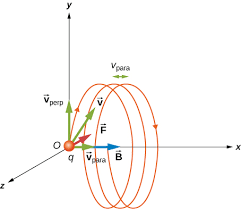
\includegraphics[width=0.3\textwidth]{pictures/4.8.1.png}
    \caption{Motion of the charged particle}
\end{figure}

\subsubsection{Aurora Borealis}
The Sun emits charged particles (ions), which we call the solar wind. When the solar wind reaches the Earth, the charged particles can become trapped 
in Earth's magnetic field. 

\begin{figure}[!h]
    \centering
    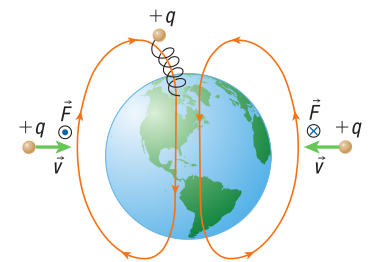
\includegraphics[width=0.3\textwidth]{pictures/4.8.2.png}
    \caption{Aurora Borealis}
\end{figure}

The ions travel along the magnetic field toward one of the poles. As they get closer to the poles, they descend into regions where the air is denser. 
When an ion collides with an air particle, such as oxygen or nitrogen, light is emitted. If enough collisions occur, the light becomes visible. 

\subsubsection{Mass Spectrometers}
Under the right conditions a particle that enters a magnetic field will undergo full \underline{uniform circular motion}\\

Following two conditions must be met:
\begin{itemize}
    \item The magnetic field must be relatively large and uniform. 
    \item The particle must be travelling perpendicular to the field. 
\end{itemize}

\textbf{Procedures}\\

Mass spectrometers can be used to determine the mass of a particle with the following steps:
\begin{itemize}
    \item A source to inject particles into the spectrometer at the correct speed.
    \item A device that causes the particles to become ionized.
    \item A particle accelerator to launch the particles into a magnetic field.
    \item A large, uniform magnetic field.
    \item A movable ion detector, used to determine where the ion emerges from the magnetic field.
\end{itemize}

\begin{theorem}
    If we can determine the charge $q$ of the particle, the magnetic field strength ($B$), the potential difference $\Delta v$, and the radius of the particle's circular motion, 
    the mass of the particle can be calculated using this formula:
    \begin{equation*}
        m = \frac{
            \left|q\right| B^2 R^2
        }{
            2 \left|\Delta v\right|
        }
    \end{equation*}
    Do not include the sign when using the formula. 
\end{theorem}

Another useful formula is:
\begin{align*}
    \Delta \vec{F} &= m\vec{a}\\
    F_M &= ma_c\\
    \left|q\right|vB\sin\theta &= m\frac{v^2}{R}
\end{align*}
